% Provenance (never printed): see sources/outline_sources.md (Year 2: effusive and explosive
% eruptions, eruptive styles, eruption columns, pyroclastic deposits, explosivity index,
% volcano monitoring).
% Curves from figdata/bachelor-2/eruptions.py (closed-system gas fraction, Cotopaxi Layer 5
% thinning, GVP frequency-size law, column height fits, Mogi uplift); exercise and problem
% values in the Book 4 scratch calculators calc/ch06.py and calc/ch06pb.py.
\chapter{ज्वालामुखी उद्गार}\label{ch:b2:eruptive-styles}

15 जून 1991 को फ़िलीपींस के माउंट पिनातूबो ने पाँच घन किलोमीटर से अधिक
पदार्थ बाहर फेंका; उसका राख-मेघ
\qty{35}{km} तक उठा, शिखर \qty{2.5}{km} चौड़े \omterm{def:b2:eruptive-styles:caldera}{कैल्डेरा} में धँस गया, और
समतापमंडल में पहुँचाई गई उसकी दो करोड़ टन सल्फ़र डाइऑक्साइड ने पूरी
पृथ्वी को दो वर्षों तक लगभग आधा डिग्री ठंडा कर दिया। एक सप्ताह पहले पृष्ठ तक पहुँचे पहले
\omterm{def:b2:magma-emplacement:magma}{मैग्मा} ने ऐसा कुछ नहीं किया था: रास्ते में अपनी अधिकांश गैस खो देने के कारण,
वह \omterm{def:b2:eruptive-styles:dome}{लावा गुंबद} के रूप में धीरे-धीरे बाहर रिसा। हवाई के किलाउआ पर
Pu`u~`\=O`\=o उद्गार ने \qty{4.4}{km^3} लावा उगला, आयतन में तुलनीय,
पैंतीस वर्षों में, फ़व्वारों और प्रवाहों के रूप में जिन्होंने 215 इमारतें नष्ट कीं,
पर कभी राख का ऊँचा स्तंभ नहीं उठाया। वही पृथ्वी, वही भौतिकी, तीन व्यवहार: उन्हें
अलग करता है कि \omterm{def:b2:magma-emplacement:magma}{मैग्मा} कितनी गैस ले जाता है, क्या वह गैस गलित को चुपचाप
छोड़ सकती है, और \omterm{def:b2:magma-emplacement:magma}{मैग्मा} कितनी तेज़ी से उठता है। यह अध्याय किसी उद्गार का
अनुसरण करता है, नलिका के बुलबुलों से छिद्र के ऊपर के स्तंभ और उसके छोड़े
निक्षेपों तक, फिर उद्गारों को मापता है, उन्हें गिनता है, और ज्वालामुखियों पर उन
संकेतों के लिए नज़र रखता है जो बताते हैं कि कोई उद्गार आने वाला है।
% ledger: usgs:pinatubo-1991, usgs:puuoo

\begin{recall}
\textbf{विद्यालयी पुस्तकों से}: ज्वालामुखी, उसका छिद्र और क्रेटर, उसके नीचे का मैग्मा-कक्ष,
लावा, और ज्वालामुखीय राख। \textbf{\cref{ch:b2:magma-emplacement}
से}: \omterm{def:b2:magma-emplacement:volatiles}{मैग्मीय वाष्पशील}, संतृप्ति दाब से नीचे उनका निर्विलयन,
जल-विलेयता का वर्गमूल नियम $w = s\sqrt p$, जिसमें
$s \approx 0.34$ प्रतिशत प्रति $\sqrt{\unit{MPa}}$ बेसाल्ट के लिए और $0.44$
रायोलाइट के लिए, और गलितों की श्यानताएँ, जो परिमाण की दस कोटियों तक भिन्न हैं।
\textbf{भौतिकी की पुस्तकों से}: आदर्श गैस नियम $pV = nRT$; उत्प्लावन;
विमीय विश्लेषण, जो दी गई राशियों का वह एकमात्र संयोजन बनाता है
जिसकी विमा उत्तर की है; प्रक्षेप्य का परास, $v^2\sin 2\theta/g$,
वायु-प्रतिरोध के बिना। \textbf{गणित की पुस्तकों से}: प्वासों प्रक्रम,
जिसमें स्थिर दर $\lambda$ पर स्वतंत्र घटनाएँ कम-से-कम एक घटना देती हैं
समय $t$ में, प्रायिकता $1 - e^{-\lambda t}$ के साथ; न्यूनतम-वर्ग सीधी रेखाएँ।
पुस्तक 3 (स्नातक वर्ष 1) से: भूकंप और उनके परिमाण।
\end{recall}

\section{बहिःस्रावी या विस्फोटक}

\begin{definition}[बहिःस्रावी और विस्फोटक उद्गार, विखंडन]\label{def:b2:eruptive-styles:regimes}
\emph{बहिःस्रावी उद्गार}\index{बहिःस्रावी उद्गार} वह है जिसमें
लावा का बहिर्प्रवाह प्रधान होता है, जो एक संसक्त द्रव के रूप में छिद्र से दूर बहता है।
\emph{विस्फोटक उद्गार}\index{विस्फोटक उद्गार} मुख्यतः खंड उत्पन्न करता है,
राख, झाँवा और प्राक्षेपिक मलबा, जिन्हें फैलती गैस ले जाती है। \emph{मैग्मा
विखंडन}\index{मैग्मा विखंडन} बुलबुलों वाले एक सतत गलित का टूटकर
गलित की बूँदें और खंड ले जाती एक सतत गैस बन जाना है;
यह बहिःस्रावी प्रवाह को विस्फोटक में बदल देता है।
\end{definition}
% ledger: usgs:glossary-ch6, cassidy18:fragmentation

संक्रमण को गैस चलाती है। गहराई से उठता \omterm{def:b2:magma-emplacement:magma}{मैग्मा} घुला हुआ जल और
कार्बन डाइऑक्साइड ले जाता है; अपने संतृप्ति दाब से नीचे वाष्पशील
विलयन से बुलबुलों के रूप में बाहर आते हैं, और दाब घटने के साथ बुलबुले फैलते हैं।
यदि वे गलित में ही रहें, तो गैस जल्दी ही आयतन का अधिकांश भाग भर देती है।

\begin{proposition}[बंद-तंत्र विगैसन में गैस का आयतन-अंश]\label{prop:b2:eruptive-styles:gas}
मान लीजिए किसी \omterm{def:b2:magma-emplacement:magma}{मैग्मा} में जल का द्रव्यमान-अंश $w_0$ है, विलेयता $w(p) =
s\sqrt p$ के साथ, और मान लीजिए कि निर्विलयित जल गलित के साथ तापमान $T$ पर
आदर्श गैस के रूप में रहता है। संतृप्ति दाब $p_s = (w_0/s)^2$ से नीचे, एक
किलोग्राम \omterm{def:b2:magma-emplacement:magma}{मैग्मा} में $x = w_0 - s\sqrt p$ किलोग्राम वाष्प होती है, और गैस का
आयतन-अंश है
\[
\phi(p) = \frac{V_g}{V_g + V_m}, \qquad V_g = \frac{x\,RT}{M p}, \qquad
V_m = \frac{1 - x}{\rho_m},
\]
जहाँ $M = \qty{0.018}{kg/mol}$ जल का मोलर द्रव्यमान है और $\rho_m$ गलित का
घनत्व।
\end{proposition}

\begin{proof}
$p_s$ से ऊपर गलित अपना सारा जल धारण कर सकता है और कोई गैस नहीं होती। $p_s$ से नीचे
गलित केवल अपनी विलेयता $s\sqrt p$ रखता है, इसलिए द्रव्यमान $x = w_0 - s\sqrt p$ प्रति
किलोग्राम \omterm{def:b2:magma-emplacement:magma}{मैग्मा} वाष्प है। वह वाष्प, $x/M$ मोल, आदर्श गैस नियम से $xRT/(Mp)$
घेरती है; गलित के शेष $1 - x$ किलोग्राम $(1 - x)/\rho_m$ घेरते हैं।
आयतन-अंश इसी से निकलता है।
\end{proof}
% ledger: moore98:h2o

चूँकि $V_g$ $1/p$ की तरह बढ़ता है, झाग पृष्ठ के निकट सबसे तेज़ी से फूलता है।
नीचे का चित्र \qty{5}{\percent} जल वाले एक रायोलाइट और \qty{1}{\percent} वाले
एक बेसाल्ट का अनुसरण करता है। रायोलाइट \qty{127}{MPa} पर संतृप्त होता है, लगभग
\qty{5}{km} नीचे; \qty{10}{MPa} पर उसकी गैस पहले ही आयतन का \qty{82}{\percent}
भर देती है। नलिका-प्रवाह के एक प्रकाशित मॉडल में \omterm{def:b2:magma-emplacement:magma}{मैग्मा} तब विखंडित होता है जब
गैस उसके आयतन का \qty{85}{\percent} भर दे, एक स्तर जिस पर यह रायोलाइट
\qty{8.2}{MPa} पर पहुँचता है, \qty{0.025}{MPa/m} की दाब-प्रवणता के लिए छिद्र से
लगभग \qty{330}{m} नीचे। बेसाल्ट केवल \qty{8.7}{MPa} पर संतृप्त होता है और वही
झाग \qty{1.8}{MPa} पर पाता है, पृष्ठ से सौ मीटर के भीतर।
% ledger: cassidy18:fragmentation, cassidy18:ascent

\begin{omfigure}
\centering
\begin{tikzpicture}
\begin{axis}[omrecord, width=0.82\linewidth, height=5.6cm, xmode=log,
  xmin=0.01, xmax=200, ymin=0, ymax=1,
  xlabel={दाब (\unit{MPa})}, ylabel={गैस का आयतन-अंश $\phi$},
  legend pos=south west, legend style={font=\scriptsize},
  tick label style={font=\scriptsize}, label style={font=\small}]
\addplot[very thick, red!70!black] table[x=p_MPa, y=rhyolite] {figdata/out/bachelor-2-eruptions-gas.dat};
\addlegendentry{रायोलाइट, \qty{5}{\percent} H$_2$O, \qty{850}{\celsius}}
\addplot[very thick, black, dashed] table[x=p_MPa, y=basalt] {figdata/out/bachelor-2-eruptions-gas.dat};
\addlegendentry{बेसाल्ट, \qty{1}{\percent} H$_2$O, \qty{1200}{\celsius}}
\draw[densely dotted, thick, gray] (axis cs:0.01,0.85) -- (axis cs:200,0.85);
\node[anchor=north west, font=\scriptsize, inner sep=1pt] at (axis cs:0.012,0.835) {एक नलिका मॉडल में विखंडन};
\end{axis}
\end{tikzpicture}
\par\smallskip{\small दाब के सापेक्ष निर्विलयित जलवाष्प का आयतन-अंश,
बंद-तंत्र विगैसन में (\cref{prop:b2:eruptive-styles:gas}), \cref{ch:b2:magma-emplacement}
के विलेयता नियमों के साथ। दाब बाईं ओर घटता है, जैसे-जैसे \omterm{def:b2:magma-emplacement:magma}{मैग्मा}
उठता है; बिंदुदार रेखा वह गैस-अंश दर्शाती है जिस पर एक प्रकाशित नलिका मॉडल
\omterm{def:b2:magma-emplacement:magma}{मैग्मा} को विखंडित करता है।}
\end{omfigure}
% ledger: moore98:h2o, cassidy18:fragmentation

तो बेसाल्ट भी विखंडित होता, यदि उसकी गैस उसमें रहती; और हवाई के लावा
फ़व्वारे में, छिद्र के निकट, वह होता भी है। अधिकांश बेसाल्टी उद्गारों को सौम्य यह बनाता है कि
गैस का रुकना आवश्यक नहीं। कम श्यानता वाले गलित में बुलबुले
द्रव में से उठते हैं, आपस में मिलते हैं और निकल जाते हैं, और जब बुलबुले एक पारगम्य जाल में जुड़ जाते हैं,
जो प्रयोगों में \qty{30}{\percent} और \qty{78}{\percent} के बीच के गैस-अंशों पर होता है,
तो गैस दीवारों और छिद्र से होकर रिस जाती है, गलित को साथ लिए
बिना: \omterm{def:b2:magma-emplacement:magma}{मैग्मा} खुले तंत्र में विगैसित होता है और पृष्ठ पर लावा के रूप में
पहुँचता है। श्यान \omterm{def:b2:magma-emplacement:magma}{मैग्मा} इसके बजाय अपने बुलबुले रोके रखता है और विखंडित होता है, गलित
काँच की तरह टूटता है जब उसे उसके बहने की क्षमता से तेज़ खींचा जाए। आरोहण-दर
दोनों के बीच उतना ही निर्णय करती है जितना संघटन: अनेक उद्गारों में, बहिःस्रावी क्रियाकलाप
लगभग \qty{0.0001}{MPa/s} की विसंपीडन-दरों के साथ जाता है और \omterm{def:b2:eruptive-styles:regimes}{विस्फोटक उद्गार}
लगभग \qty{1}{MPa/s} की दरों के साथ, और गलित की श्यानता में आधी
लघुगणकीय इकाई का परिवर्तन, लगभग तीन का गुणक, किसी उद्गार को एक व्यवस्था से
दूसरी में झुका सकता है। पिनातूबो का पहला \omterm{def:b2:eruptive-styles:dome}{लावा गुंबद} और एक सप्ताह बाद का उसका चरम उद्गार
एक ही \omterm{def:b2:magma-emplacement:magma}{मैग्मा} थे: पहले खेप को अपनी गैस खोने का समय मिला, अगले को नहीं।
% ledger: cassidy18:fragmentation, cassidy18:ascent, usgs:pinatubo-1991

बाहर का जल वही करता है जो \omterm{def:b2:magma-emplacement:magma}{मैग्मा} की अपनी गैस करती है। भूजल, कोई झील या
समुद्र जो \omterm{def:b2:magma-emplacement:magma}{मैग्मा} से मिलता है, तुरंत भाप बन जाता है, और अतितप्त
जल का प्रसार \omterm{def:b2:magma-emplacement:magma}{मैग्मा} को चकनाचूर कर देता है: प्रयोग दिखाते हैं कि उपलब्ध ऊष्मा का
\qty{30}{\percent} से अधिक यांत्रिक ऊर्जा में बदल सकता है। तब गैस में निर्धन \omterm{def:b2:magma-emplacement:magma}{मैग्मा} भी
विस्फोटक रूप से उद्गार कर सकता है।
% ledger: cassidy18:fragmentation

\section{उद्गार-शैलियाँ}

ज्वालामुखीविज्ञानी उद्गारों के नाम क्लासिक उदाहरणों पर रखते हैं। ये नाम बताते हैं कि
उद्गार कैसा दिखता है, और वे एक-दूसरे में क्रमशः घुल-मिल जाते हैं; एक ही उद्गार प्रायः
कई शैलियों से गुज़रता है।

\begin{definition}[उद्गार-शैलियाँ]\label{def:b2:eruptive-styles:styles}
बढ़ती विस्फोटकता के क्रम में, \omterm{def:b2:magma-emplacement:magma}{मैग्मा} की अपनी गैस से चलने वाले उद्गारों में:
\begin{itemize}
\item \emph{हवाईयन उद्गार}\index{हवाईयन उद्गार} अत्यंत तरल बेसाल्टी लावा के
फ़व्वारे उत्पन्न करता है, दसियों से सैकड़ों मीटर ऊँचे, जो लावा-प्रवाहों को पोषित करते हैं;
\item \emph{स्ट्रॉम्बोलियन उद्गार}\index{स्ट्रॉम्बोलियन उद्गार} अलग-अलग
विस्फोटों की एक शृंखला है जो बेसाल्टी से
बेसाल्टी-एंडेसाइट \omterm{def:b2:magma-emplacement:magma}{मैग्मा} के तप्त-दीप्त लोंदे लगभग सौ मीटर तक फेंकती है, बिना किसी सतत
स्तंभ के;
\item \emph{वल्कनियन उद्गार}\index{वल्कनियन उद्गार} जमे हुए लावा के एक डाट के नीचे
संचित गैस का एक छोटा, उग्र विस्फोट है, जो
डाट को चकनाचूर करके खंड और महीन राख का एक काला स्तंभ बाहर फेंकता है, प्रायः
मध्यवर्ती \omterm{def:b2:magma-emplacement:magma}{मैग्मा} से;
\item \emph{प्लिनियन उद्गार}\index{प्लिनियन उद्गार} गैस और विखंडित, प्रायः
सिलिसिक, \omterm{def:b2:magma-emplacement:magma}{मैग्मा} का एक सतत जेट है जो घंटों से दिनों तक समतापमंडल में
उठते स्तंभ को पोषित करता है और हज़ारों वर्ग किलोमीटर पर झाँवा और राख की
एक चादर फैलाता है।
\end{itemize}
जहाँ बाहरी जल विखंडन चलाता है, वहाँ \emph{फ़्रीएटोमैग्मीय
उद्गार}\index{फ़्रीएटोमैग्मीय उद्गार} भाप के साथ ताज़े \omterm{def:b2:magma-emplacement:magma}{मैग्मा} के खंड
बाहर फेंकता है, जबकि \emph{फ़्रीएटिक उद्गार}\index{फ़्रीएटिक उद्गार}
\omterm{def:b2:magma-emplacement:magma}{मैग्मा} या गरम चट्टान से गरम हुए भूजल या पृष्ठ-जल का भाप-चालित विस्फोट है,
जो भाप और पुरानी चट्टान के खंड फेंकता है, पर कोई ताज़ा \omterm{def:b2:magma-emplacement:magma}{मैग्मा} नहीं।
\end{definition}
% ledger: nps:styles, usgs:glossary-ch6

हर शैली के अपने प्रतिरूपी उद्गार हैं। किलाउआ पर Pu`u~`\=O`\=o अपने
पैंतीस वर्षों और इकसठ प्रकरणों के अधिकांश समय हवाईयन रहा, ऐसे फ़व्वारों के साथ जो प्रायः
\qtyrange{10}{100}{m} और कभी-कभी \qty{500}{m} से अधिक उठे। स्ट्रॉम्बोली,
``भूमध्यसागर का प्रकाशस्तंभ'', ने अपना नाम उन विस्फोटों को दिया है जो
सिंडर शंकु बनाते हैं। वल्कनियन विस्फोटों ने अलास्का के ट्राइडेंट को
1953 और 1974 के बीच रुक-रुककर हिलाया। सन्~79 में विसूवियस, जिसका वर्णन कनिष्ठ प्लिनी ने किया, ने
प्लिनियन उद्गारों को अपना नाम दिया; 18~मई~1980 को माउंट सेंट~हेलेंस और 1912 में नोवारुप्ता,
जिसका स्तंभ लगभग तीन दिन चले उद्गार में \qty{30}{km} से ऊपर उठा,
आधुनिक उदाहरण हैं।
लगभग \qty{20}{km} से नीचे के स्तंभों वाले मध्यवर्ती मामले, सतत पर अस्थिर,
उप-प्लिनियन कहलाते हैं। जल के साथ \omterm{def:b2:eruptive-styles:styles}{स्ट्रॉम्बोलियन उद्गार} सर्टसियन बन जाता है,
आइसलैंड के तट के पास सर्टसी के 1963 के उद्गार के नाम पर, और टफ़ के
निचले वलय और मार बनाता है; \omterm{def:b2:eruptive-styles:styles}{प्लिनियन उद्गार} फ़्रीएटोप्लिनियन बन जाता है। पिनातूबो पर,
भाप-विस्फोटों ने मार्च और अप्रैल 1991 में उत्तरी ढाल पर तीन क्रेटर उड़ा दिए, चरम उद्गार से
दो महीने पहले: वे फ़्रीएटिक थे।
% ledger: nps:styles, usgs:puuoo, usgs:glossary-ch6, usgs:pinatubo-deposits

\begin{definition}[लावा गुंबद]\label{def:b2:eruptive-styles:dome}
\emph{लावा गुंबद}\index{लावा गुंबद} श्यान लावा का खड़ी ढालों वाला टीला है,
प्रायः डेसाइट या रायोलाइट, जो किसी छिद्र से धीरे-धीरे बाहर निकलकर उसके ऊपर ढेर हो जाता है,
दूर बहने के बजाय।
\end{definition}
% ledger: usgs:glossary-ch6

गुंबद वह हैं जो श्यान \omterm{def:b2:magma-emplacement:magma}{मैग्मा} अपनी गैस खो देने पर बनाता है: जून 1991 में पिनातूबो का पहला
\omterm{def:b2:magma-emplacement:magma}{मैग्मा}, और वह गुंबद जो माउंट सेंट~हेलेंस के क्रेटर में 1980 और 1986 के बीच
सत्रह प्रकरणों में क्रेटर-तल से \qty{267}{m} ऊपर तक बढ़ा।
गुंबद वह डाट भी हो सकता है जिसके नीचे अगला वल्कनियन विस्फोट तैयार होता है,
और उसका ढहना नीचे के गैस-समृद्ध \omterm{def:b2:magma-emplacement:magma}{मैग्मा} पर दाब मुक्त कर सकता है। नीचे के
फ़ोटो इस परास के दोनों छोर दिखाते हैं।
% ledger: usgs:pinatubo-1991, usgs:msh-dome, cassidy18:fragmentation

\begin{omfigure}
\centering
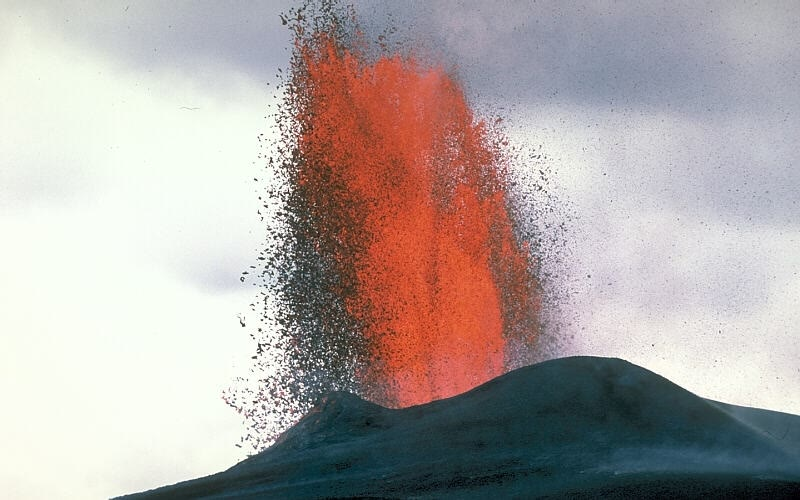
\includegraphics[height=4.3cm]{images/book4/b2-kilauea-fountain.jpg}\hfill
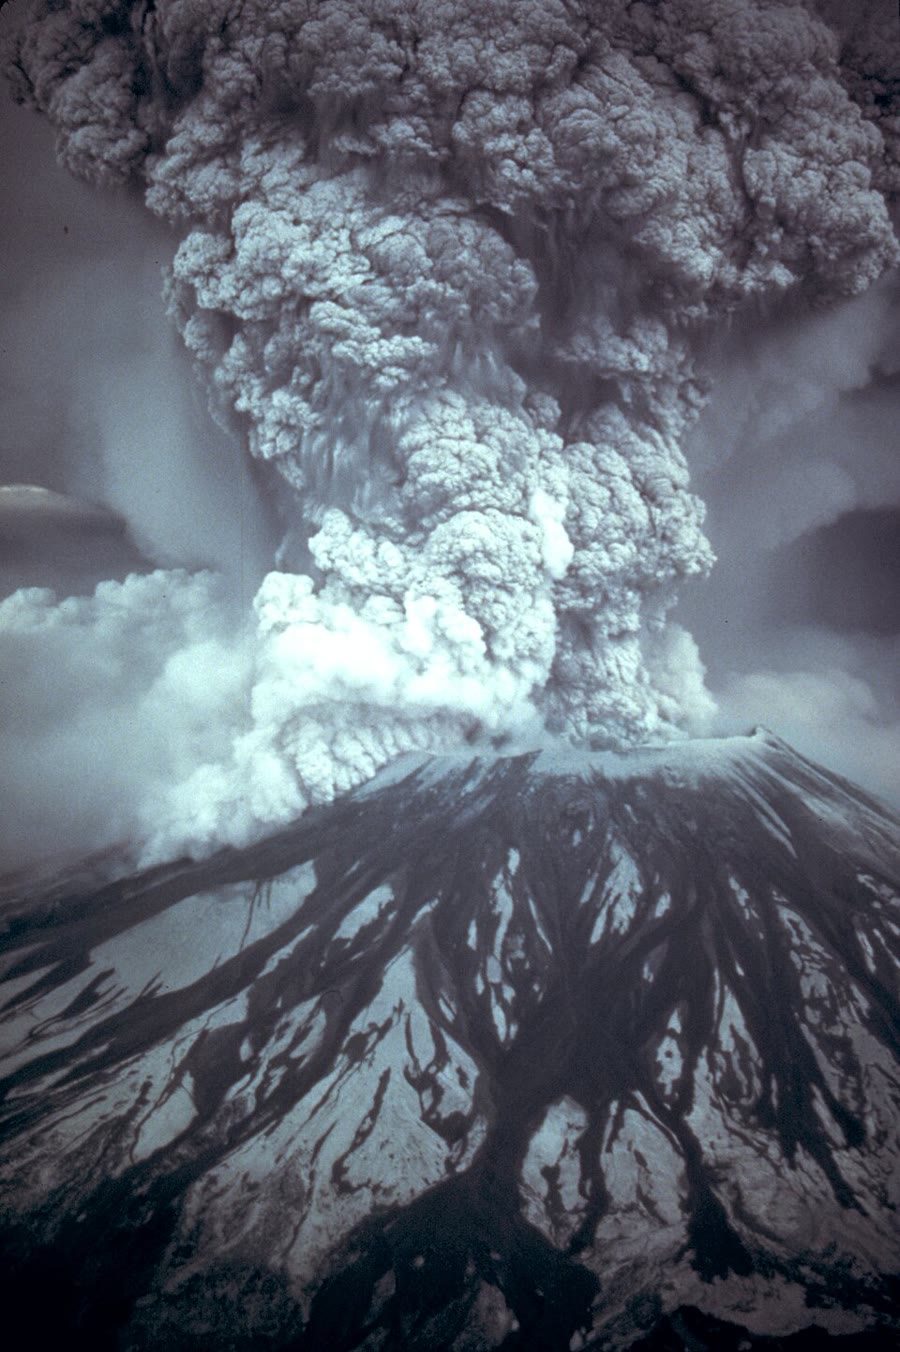
\includegraphics[height=4.3cm]{images/book4/b2-st-helens-column.jpg}\hfill
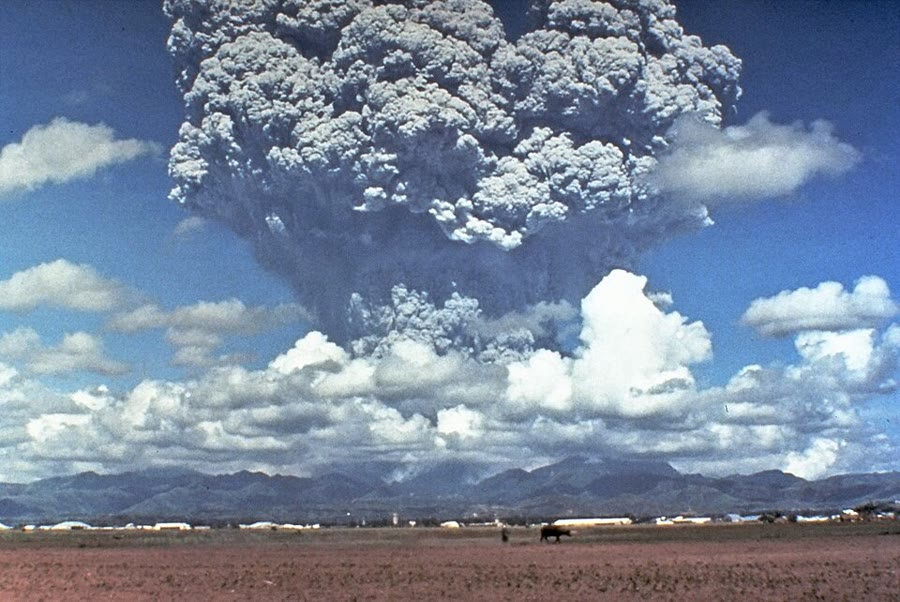
\includegraphics[height=4.3cm]{images/book4/b2-pinatubo-column.jpg}
\par\smallskip{\small बाएँ: किलाउआ के Pu`u~`\=O`\=o शंकु पर एक हवाईयन फ़व्वारा,
अक्टूबर 1983 (फ़ोटो: J.\,D.~Griggs, USGS)। मध्य: माउंट सेंट~हेलेंस का प्लिनियन स्तंभ,
18 मई 1980 (फ़ोटो: Austin Post, USGS)। दाएँ: 12 जून 1991 को माउंट पिनातूबो का
\omterm{def:b2:eruptive-styles:column}{उद्गार-स्तंभ}, चरम उद्गार से तीन दिन पहले (फ़ोटो: Dave Harlow, USGS)। तीनों
फ़ोटो सार्वजनिक डोमेन में हैं।}
\end{omfigure}
% ledger: usgs:puuoo, usgs:msh-may18, usgs:pinatubo-1991

\section{उद्गार-स्तंभ}

\begin{definition}[उद्गार-स्तंभ]\label{def:b2:eruptive-styles:column}
\emph{उद्गार-स्तंभ}\index{उद्गार-स्तंभ} किसी विस्फोटक छिद्र के ऊपर गैस और
खंडों का आरोही द्रव्यमान है। इसके तीन भाग हैं: \emph{जेट}, या
गैस-प्रणोद क्षेत्र, जिसमें मिश्रण छिद्र से तेज़ी से पर वायु से सघन
निकलता है और अपने संवेग से उठता है; \emph{संवहनी} क्षेत्र, जिसमें मिश्रण,
अपने परिवेश से हल्का होने लायक वायु को निगलकर और गरम करके,
उत्प्लावन से उठता है; और \emph{छत्र} मेघ, जो उस स्तर पर किनारों की ओर फैलता है
जहाँ स्तंभ का घनत्व वायुमंडल के घनत्व के बराबर होता है।
\end{definition}
% ledger: usgs:glossary-ch6, nps:styles, aubry23:fits

\begin{omfigure}
\centering
\begin{tikzpicture}[x=1cm, y=1cm, font=\scriptsize]
% atmosphere and ground
\fill[blue!6] (-6.2,0) rectangle (6.2,6.4);
% volcano
\fill[brown!45, draw=brown!70!black] (-4.8,0) -- (-0.45,1.6) -- (0.45,1.6) -- (4.8,0) -- cycle;
% collapse branch (left): a density current hugging the flank
\fill[gray!55] (-0.45,1.6) -- (-0.7,2.35) .. controls (-1.1,2.25) and (-1.5,1.65) .. (-2.2,1.3)
  .. controls (-3.4,0.85) and (-4.6,0.42) .. (-5.9,0.28) -- (-5.9,0) -- (-4.8,0) -- cycle;
% jet
\fill[gray!70] (-0.45,1.6) -- (0.45,1.6) -- (0.75,2.5) -- (-0.75,2.5) -- cycle;
% convective column
\fill[gray!45] (-0.75,2.5) .. controls (-1.1,3.2) and (-1.0,3.8) .. (-1.4,4.2)
  -- (1.4,4.2) .. controls (1.0,3.8) and (1.1,3.2) .. (0.75,2.5) -- cycle;
% umbrella
\fill[gray!35] (-1.4,4.2) .. controls (-3,4.1) and (-5,4.2) .. (-5.8,4.45)
  .. controls (-5,4.9) and (-3,5.1) .. (0,5.25) .. controls (3,5.1) and (5,4.9) .. (5.8,4.45)
  .. controls (5,4.2) and (3,4.1) .. (1.4,4.2) -- cycle;
\draw[densely dashed, blue!60!black] (-6.2,4.4) -- (6.2,4.4);
% fallout from the far end of the umbrella, down to the ground
\foreach \x in {4.95,5.25,5.55} {\draw[gray!70, densely dotted, thick] (\x,4.3) -- (\x-0.1,0.02);}
\draw[gray, densely dotted] (0.45,1.6) -- (6.0,1.6);
\draw[<->] (6.0,1.6) -- (6.0,5.25) node[midway, right, align=left] {शीर्ष\\ऊँचाई\\$H$\\छिद्र के\\ऊपर};
% labels
\node[anchor=north west, align=left, blue!60!black] at (-6.1,4.3) {उदासीन उत्प्लावकता\\का स्तर (डैश)};
\draw (-0.95,3.3) -- (-1.8,3.05) node[left, align=right] {संवहनी क्षेत्र:\\उत्प्लावक, वायु खींचता है};
\draw (0.3,2.05) -- (2.0,2.35) node[right, align=left] {जेट: संवेग,\\वायु से सघन};
\draw (2.6,4.85) -- (3.2,5.75) node[right] {छत्र मेघ};
\node[anchor=east, align=right] at (4.8,1.25) {छत्र से\\अवपात};
\draw (-3.4,0.7) -- (-3.9,1.5) node[above, align=center] {ढहना: पायरोक्लास्टिक\\घनत्व धारा};
\draw[-latex] (0,1.0) -- (0,1.55);
\node[anchor=north] at (0,1.0) {छिद्र};
\end{tikzpicture}
\par\smallskip{\small \omterm{def:b2:eruptive-styles:column}{उद्गार-स्तंभ} की संरचना (व्यवस्था-चित्र, पैमाने के अनुसार नहीं)।
दाईं ओर स्तंभ अपने तीन क्षेत्रों से होकर उठता है और छत्र मेघ फैलते हुए
\omterm{def:b2:eruptive-styles:tephra}{टेफ़्रा} गिराता है; बाईं ओर जेट का एक भाग उत्प्लावक नहीं बन पाया
और ढहकर \omterm{def:b2:eruptive-styles:pdc}{पायरोक्लास्टिक घनत्व धारा} बन जाता है।}
\end{omfigure}

स्तंभ कितना ऊँचा उठता है, यह सबसे बढ़कर इस पर निर्भर करता है कि वह प्रति सेकंड कितनी ऊष्मा
लाता है, अर्थात द्रव्यमान उद्गार-दर~$Q$ पर। विमीय विश्लेषण
नियम का रूप देता है।

\begin{proposition}[उत्प्लावक प्लूम की ऊँचाई]\label{prop:b2:eruptive-styles:plume}
यदि किसी स्थिर बिंदु-स्रोत के ऊपर उत्प्लावक प्लूम की शीर्ष ऊँचाई $H$ केवल
स्रोत के उत्प्लावन-फ़्लक्स $F$ (विमा $\mathrm{m^4\,s^{-3}}$) और
स्थिर रूप से स्तरित वायुमंडल की उत्प्लावन-आवृत्ति $N$ (विमा
$\mathrm{s^{-1}}$) पर निर्भर करती है, तो
\[
H = c\,F^{1/4}N^{-3/4}
\]
जहाँ $c$ एक विमाहीन स्थिरांक है। चूँकि $F$ ऊष्मा-फ़्लक्स के, और इसलिए
द्रव्यमान उद्गार-दर के, समानुपाती है, किसी दिए गए वायुमंडल में $H \propto Q^{1/4}$।
\end{proposition}

\begin{proof}
$H = c\,F^{\alpha}N^{\beta}$ लिखिए। लंबाइयों का मिलान $4\alpha = 1$ देता है; समयों का
मिलान $-3\alpha - \beta = 0$ देता है। अतः $\alpha = 1/4$ और $\beta = -3/4$, और
$F$ और $N$ का कोई अन्य संयोजन लंबाई की विमा नहीं रखता।
\end{proof}

स्थिरांक $c$ इससे आता है कि प्लूम कितनी तेज़ी से वायु निगलता है, जिसे प्लूम-सिद्धांत
प्रयोगों में मापे गए एक अंतर्ग्रहण गुणांक से संभालता है; उसे यहाँ स्वीकार किया
जाता है। वास्तविक स्तंभ शांत वायुमंडल में स्थिर बिंदु-स्रोत नहीं होते, इसलिए
ज्वालामुखीविज्ञानी इस नियम को उन उद्गारों पर बिठाते हैं जिनकी ऊँचाई और द्रव्यमान उद्गार-दर
दोनों मापी गई थीं।
% ledger: aubry23:fits

\begin{proposition}[स्तंभ की ऊँचाई और द्रव्यमान उद्गार-दर]\label{prop:b2:eruptive-styles:mastin}
किलोमीटर में छिद्र के ऊपर शीर्ष ऊँचाई $H$ और किलोग्राम प्रति सेकंड में द्रव्यमान उद्गार-दर
$Q$ के लिए, सुप्रलेखित उद्गारों का संकलन देता है
\[
H = 0.304\,Q^{0.241},
\]
और 130 घटनाओं का एक बड़ा, स्वतंत्र डेटा-समुच्चय $H = 0.345\,Q^{0.226}$ देता है।
प्रकीर्णन बड़ा है: $H$ पर सापेक्ष वर्ग-माध्य-मूल त्रुटि
\qtyrange{53}{60}{\percent} है।
\end{proposition}
\admitted
% ledger: aubry23:fits

दोनों घातांक प्लूम-सिद्धांत के $1/4$ के निकट हैं। नीचे का चित्र
दोनों फ़िट और वे उदाहरण-उद्गार दिखाता है जिन पर राख-पूर्वानुमान केंद्रों द्वारा प्रयुक्त
स्रोत-प्राचल आधारित हैं। माउंट सेंट~हेलेंस जैसा
\qty{15}{km} ऊँचा स्तंभ \qty{e7}{kg/s} माँगता है, हर सेकंड दस हज़ार टन; ऊँचाई
दोगुनी करने के लिए लगभग अठारह गुनी दर चाहिए। उलटे पढ़ें तो मापी गई ऊँचाई
दर देती है, पर केवल कई के गुणक के भीतर, क्योंकि $Q$ $H^4$ की तरह चलता है
(\cref{exo:b2:eruptive-styles:3})। ज्वालामुखीविज्ञानी दर को \emph{तीव्रता} $I =
\log_{10}Q + 3$ से व्यक्त करते हैं, $Q$ किलोग्राम प्रति सेकंड में।
% ledger: mastin09:examples, aubry23:fits, brown14:record

\begin{omfigure}
\centering
\begin{tikzpicture}
\begin{axis}[omrecord, width=0.82\linewidth, height=6cm, xmode=log, ymode=log,
  xmin=1e3, xmax=1e9, ymin=1, ymax=60,
  xlabel={द्रव्यमान उद्गार-दर $Q$ (\unit{kg/s})}, ylabel={छिद्र के ऊपर शीर्ष ऊँचाई (\unit{km})},
  ytick={1,2,5,10,20,50}, yticklabels={1,2,5,10,20,50},
  legend pos=north west, legend style={font=\scriptsize},
  tick label style={font=\scriptsize}, label style={font=\small}]
\addplot[very thick, black] table[x=Q, y=mastin] {figdata/out/bachelor-2-eruptions-column.dat};
\addlegendentry{$H = 0.304\,Q^{0.241}$}
\addplot[thick, red!70!black, dashed] table[x=Q, y=aubry] {figdata/out/bachelor-2-eruptions-column.dat};
\addlegendentry{$H = 0.345\,Q^{0.226}$}
\addplot[only marks, mark=*, mark size=1.8pt, blue!70!black]
  table[x=Q, y=H] {figdata/out/bachelor-2-eruptions-column-data.dat};
\addlegendentry{उदाहरण-उद्गार}
\begin{scope}[font=\tiny, inner sep=1.5pt]
\node[anchor=north west] at (axis cs:5e3,2) {एटना 2001};
\node[anchor=south east] at (axis cs:1e5,7) {सेरो नेग्रो 1992};
\node[anchor=north west] at (axis cs:2e5,5) {रुआपेहू 1996};
\node[anchor=east] at (axis cs:1e6,10) {फ़्यूएगो 1974};
\draw[gray] (axis cs:3e6,10) -- (axis cs:2e7,4.5) node[anchor=west, black] {सूफ़्रियेर हिल्स};
\draw[gray] (axis cs:4e6,11) -- (axis cs:2e7,6.5) node[anchor=west, black] {स्पर 1992};
\node[anchor=south east] at (axis cs:1e7,15) {सेंट हेलेंस 1980};
\node[anchor=south east, align=right] at (axis cs:1e8,25) {सेंट हेलेंस\\सह-इग्निम्ब्राइट};
\end{scope}
\end{axis}
\end{tikzpicture}
\par\smallskip{\small द्रव्यमान उद्गार-दर के सापेक्ष छिद्र के ऊपर उद्गार-स्तंभों की शीर्ष ऊँचाई:
Mastin और अन्य (2009) का आनुभविक फ़िट, एक स्वतंत्र डेटा-समुच्चय पर
Aubry और अन्य (2023) का फ़िट, और पहले संकलन के उदाहरण-उद्गार
(माउंट सेंट~हेलेंस का \omterm{def:b2:eruptive-styles:pdc}{सह-इग्निम्ब्राइट} मेघ छिद्र से नहीं,
\omterm{def:b2:eruptive-styles:pdc}{पायरोक्लास्टिक प्रवाहों} से उठा था)।}
\end{omfigure}
% ledger: aubry23:fits, mastin09:examples

स्तंभ उठने में विफल भी हो सकता है। जेट छिद्र से वायु से सघन निकलता है; यदि
उत्प्लावक बनने लायक वायु निगलने से पहले ही उसका संवेग चुक जाए, उदाहरण के लिए
इसलिए कि उसकी गैस-मात्रा घट जाती है, तो स्तंभ ढह जाता है और मिश्रण
एक गरम, सघन धारा के रूप में ढालों से नीचे बहता है। प्लिनियन स्तंभ
इस तरह ढह सकते हैं, और पिनातूबो पर 1991 के \omterm{def:b2:eruptive-styles:pdc}{पायरोक्लास्टिक प्रवाहों} ने घाटियों को
\qty{200}{m} तक मोटे निक्षेपों से भर दिया।
% ledger: nps:styles, usgs:pinatubo-deposits

\section{पायरोक्लास्टिक उत्पाद}

\begin{definition}[टेफ़्रा और पायरोक्लास्ट]\label{def:b2:eruptive-styles:tephra}
\emph{पायरोक्लास्ट}\index{पायरोक्लास्ट} \omterm{def:b2:magma-emplacement:magma}{मैग्मा} या उसके आसपास की चट्टानों के विस्फोटक
विखंडन से उत्पन्न खंड है। \emph{टेफ़्रा}\index{टेफ़्रा} हवा में फेंके गए
सभी पायरोक्लास्टों का सामूहिक नाम है, उनका आकार कुछ भी हो।
आकार के अनुसार, \qty{2}{mm} से महीन पायरोक्लास्ट ज्वालामुखीय राख बनाते हैं;
\qtyrange{2}{64}{mm} वाले \emph{लैपिली}\index{लैपिली} हैं;
\qty{64}{mm} से बड़े खंड ब्लॉक कहलाते हैं यदि वे फेंके जाते समय ठोस और कोणीय थे, और
\emph{ज्वालामुखीय बम}\index{ज्वालामुखीय बम} यदि वे पूर्णतः या अंशतः गलित थे
और उड़ान में गोल या तकुए जैसा आकार ले लिया।
\end{definition}
% ledger: nps:pyroclast-sizes, usgs:glossary-ch6

\omterm{def:b2:eruptive-styles:tephra}{टेफ़्रा} छत्र मेघ और स्तंभ से हवा की दिशा में एक अवपात-निक्षेप के रूप में गिरता है
जो भूमि को ढक देता है: छिद्र के निकट मोटा, उससे दूर पतला और महीन। उसकी
मोटाई \emph{समस्थूलता-रेखाओं} (समान मोटाई की रेखाओं) से मानचित्रित की जाती है, और, नियमतः,
दूरी के साथ चरघातांकी रूप से घटती है। चूँकि हवा समस्थूलता-रेखाओं को खींचकर
दीर्घवृत्त बना देती है, दूरी को हर समस्थूलता-रेखा द्वारा घेरे गए क्षेत्रफल के वर्गमूल से
मापना सबसे अच्छा है।
% ledger: usgs:ash-props, biass19:layer5

\begin{proposition}[चरघातांकी रूप से पतले होते निक्षेप का आयतन]\label{prop:b2:eruptive-styles:thinning}
यदि किसी अवपात-निक्षेप की मोटाई समस्थूलता-क्षेत्रफल के वर्गमूल $x = \sqrt A$ के साथ
$T = T_0\,e^{-kx}$ के अनुसार घटती है, तो उसका स्थूल आयतन है
\[
V = \frac{2T_0}{k^2}.
\]
उस आयतन का आधा समस्थूलता-रेखा $x_{1/2} = 1.678/k$ से परे पड़ता है।
\end{proposition}

\begin{proof}
क्षेत्रफल $A$ और $A + dA$ वाली समस्थूलता-रेखाओं के बीच निक्षेप का आयतन $T\,dA$ है,
और $dA = 2x\,dx$। इसलिए $V = \int_0^\infty T_0e^{-kx}\,2x\,dx = 2T_0/k^2$,
खंडशः समाकलन से ($\int_0^\infty xe^{-kx}dx = 1/k^2$)। $x$ के भीतर का आयतन
$\frac{2T_0}{k^2}[1 - (1 + kx)e^{-kx}]$ है, जो कुल का आधा तब होता है जब $(1 +
u)e^{-u} = 1/2$, $u = kx$ के साथ, अर्थात $u = 1.678$।
\end{proof}

वास्तविक निक्षेप दो या अधिक ढालों के साथ पतले होते हैं, छिद्र के निकट खड़ी और दूर
धीमी, क्योंकि मोटे \omterm{def:b2:eruptive-styles:tephra}{लैपिली} स्तंभ से तेज़ी से गिरते हैं और महीन राख
बहती चली जाती है। हर खंड अलग से फ़िट किया जाता है और समाकल खंड-दर-खंड
लिया जाता है।

\begin{method}[समस्थूलता-रेखाओं से अवपात-निक्षेप का आयतन]\label{met:b2:eruptive-styles:volume}
हर समस्थूलता-रेखा के लिए $\ln T$ को $\sqrt A$ के सापेक्ष आलेखित कीजिए और संरेखित बिंदुओं की हर
शृंखला पर एक सीधी रेखा बिठाइए। दो खंडों के लिए, $T_0e^{-k_1x}$ दोनों रेखाओं के
प्रतिच्छेद-बिंदु $X$ के भीतर और दूसरी उसके परे, आयतन है
\[
V = \frac{2T_0}{k_1^2} + 2T_0e^{-k_1X}\left[\frac{k_2X + 1}{k_2^2} -
\frac{k_1X + 1}{k_1^2}\right]
\]
(\cref{exo:b2:eruptive-styles:10})। स्थूल आयतन को सघन-शैल समतुल्य में बदलिए, जो
उसी द्रव्यमान का बुलबुला-रहित \omterm{def:b2:magma-emplacement:magma}{मैग्मा} के रूप में आयतन है: $V_{\mathrm{DRE}} = V\rho_{\mathrm{deposit}}/\rho_{\mathrm{magma}}$।
\end{method}
% ledger: biass19:layer5, brown14:record

नीचे का चित्र यह विधि इक्वाडोर के कोटोपैक्सी द्वारा लगभग \num{1200} वर्ष पहले
उगले गए एक स्कोरिया-अवपात पर लागू करता है। दो खंड छह समस्थूलता-रेखाओं पर बैठते हैं,
\qty{1.9}{km} और \qty{5.0}{km} की मोटाई-अर्धदूरियों $\ln 2/k$ के साथ (वह
प्रकाशित अध्ययन, जिसका फ़िट थोड़ा भिन्न है, \qty{1.9}{km} और
\qty{5.3}{km} पाता है), और आयतन \qty{0.29}{km^3} आता है, जैसा उस अध्ययन में। इसका
\qty{40}{\percent} से अधिक पतले दूरस्थ खंड में पड़ता है, इसीलिए दूरस्थ राख,
जो आसानी से अपरदित होती है या कभी मानचित्रित नहीं होती, कुल के लिए इतनी महत्त्वपूर्ण है। ताज़ा गिरी राख
का स्थूल घनत्व \qtyrange{500}{1500}{kg/m^3} है, \omterm{def:b2:magma-emplacement:magma}{मैग्मा} के घनत्व से काफ़ी
नीचे, इसलिए सघन-शैल समतुल्य मोटे तौर पर स्थूल आयतन का आधा या उससे कम होता है।
% ledger: biass19:layer5, usgs:ash-props

\begin{omfigure}
\centering
\begin{tikzpicture}
\begin{axis}[omrecord, width=0.78\linewidth, height=5.6cm, ymode=log,
  xmin=0, xmax=30, ymin=2, ymax=2000,
  xlabel={$\sqrt{\text{समस्थूलता-क्षेत्रफल}}$ (\unit{km})}, ylabel={मोटाई (\unit{cm})},
  ytick={2,5,10,20,50,100,200,500,1000,2000}, yticklabels={2,5,10,20,50,100,200,500,1000,2000},
  legend pos=north east, legend style={font=\scriptsize},
  tick label style={font=\scriptsize}, label style={font=\small}]
\addplot[thick, black, restrict x to domain=0:12] table[x=sqrtA_km, y=seg1] {figdata/out/bachelor-2-eruptions-thin-fit.dat};
\addlegendentry{निकटस्थ खंड, $k_1 = \qty{0.365}{km^{-1}}$}
\addplot[thick, red!70!black, dashed, restrict x to domain=5:30] table[x=sqrtA_km, y=seg2] {figdata/out/bachelor-2-eruptions-thin-fit.dat};
\addlegendentry{दूरस्थ खंड, $k_2 = \qty{0.138}{km^{-1}}$}
\addplot[only marks, mark=*, mark size=2pt, blue!70!black] table[x=sqrtA_km, y=T_cm] {figdata/out/bachelor-2-eruptions-thin-data.dat};
\addlegendentry{समस्थूलता-रेखाएँ}
\end{axis}
\end{tikzpicture}
\par\smallskip{\small कोटोपैक्सी (इक्वाडोर) की लगभग \num{1200} वर्ष पुरानी परत~5
के स्कोरिया-अवपात का पतला होना: समस्थूलता-मोटाइयाँ Biass, Bonadonna और
Houghton (2019) से, हर समस्थूलता-रेखा द्वारा घेरे क्षेत्रफल के वर्गमूल के सापेक्ष (ऊर्ध्वाधर
पैमाना लघुगणकीय है)। दो चरघातांकी खंड, दो
निकटस्थ और चार दूरस्थ समस्थूलता-रेखाओं पर बिठाए गए, $\sqrt A = \qty{8.6}{km}$ पर काटते हैं;
समाकलित करने पर वे \qty{0.29}{km^3} का स्थूल आयतन देते हैं।}
\end{omfigure}
% ledger: biass19:layer5

सारा \omterm{def:b2:eruptive-styles:tephra}{टेफ़्रा} आकाश से नहीं गिरता। जब कोई स्तंभ ढहता है, कोई गुंबद भुरभुराता है या कोई
पार्श्व विस्फोट ज्वालामुखी का पार्श्व फाड़ देता है, तो गरम मिश्रण भूमि के अनुदिश
दौड़ता है।

\begin{definition}[पायरोक्लास्टिक घनत्व धाराएँ]\label{def:b2:eruptive-styles:pdc}
\emph{पायरोक्लास्टिक घनत्व धारा}\index{पायरोक्लास्टिक घनत्व धारा} गरम गैस और
\omterm{def:b2:eruptive-styles:tephra}{पायरोक्लास्टों} का भूमि से सटा मिश्रण है जो ढाल पर नीचे या बाहर की ओर बहता है
क्योंकि वह वायु से सघन है। \emph{पायरोक्लास्टिक प्रवाह}\index{पायरोक्लास्टिक प्रवाह}
चट्टान-खंडों, राख और गैस की एक सांद्र धारा है, सामान्यतः
\qtyrange{200}{700}{\celsius} पर, जो दसियों मीटर प्रति सेकंड से चलती है;
\emph{पायरोक्लास्टिक उफान}\index{पायरोक्लास्टिक उफान} राख,
चट्टान और गैस का अधिक तनु मेघ है, कई सौ डिग्री का, जो हरिकेन
पवन की चाल से चलता है। \emph{इग्निम्ब्राइट}\index{इग्निम्ब्राइट} पायरोक्लास्टिक
घनत्व धाराओं द्वारा निक्षेपित चट्टान है, जो अपनी ही ऊष्मा से वेल्डित हो सकती है।
\end{definition}
% ledger: usgs:glossary-ch6

18 मई 1980 को माउंट सेंट~हेलेंस की उत्तरी ढाल के ढहने ने, जो लगभग \qty{2.8}{km^3}
के साथ दर्ज इतिहास का सबसे बड़ा भूस्खलन था, \omterm{def:b2:magma-emplacement:magma}{मैग्मा} की छत उघाड़ दी और
एक पार्श्व विस्फोट छोड़ा जो
\qty{480}{km/h} तक की चाल से लगभग \qty{600}{km^2} पर फैला; फिर कम-से-कम \qty{700}{\celsius} के \omterm{def:b2:eruptive-styles:pdc}{पायरोक्लास्टिक प्रवाह}
क्रेटर से \qty{8}{km} तक पहुँचे। पिनातूबो के 1991 के प्रवाह पाँच वर्ष बाद भी भीतर
\qty{500}{\celsius} तक गरम थे।
% ledger: usgs:msh-may18, usgs:msh-flows, usgs:msh-reach, usgs:pinatubo-deposits

\begin{definition}[लाहार]\label{def:b2:eruptive-styles:lahar}
\emph{लाहार}\index{लाहार} जल और ज्वालामुखीय मलबे का तेज़ी से चलता मिश्रण है
जो नदी-घाटी में नीचे बहता है, जिसकी गाढ़ता गंदले पानी से लेकर
गीले कंक्रीट तक कुछ भी हो सकती है। लाहार तब बनते हैं जब पायरोक्लास्टिक धाराएँ हिम और बर्फ़ पिघलाती हैं, जब
ढीले ज्वालामुखीय निक्षेपों पर भारी वर्षा होती है, जब ज्वालामुखीय
निक्षेपों से बँधी कोई झील टूटकर बहती है, या किसी मलबा-हिमस्खलन से।
\end{definition}
% ledger: usgs:glossary-ch6

\omterm{def:b2:eruptive-styles:lahar}{लाहार} उद्गारों से अधिक समय तक रहते हैं। पिनातूबो के आसपास मानसून और टाइफ़ून की वर्षा ने
1991 की राख को वर्षों तक \omterm{def:b2:eruptive-styles:lahar}{लाहारों} में बदला, और उन्होंने स्वयं
उद्गार से अधिक विनाश किया।
% ledger: usgs:pinatubo-lahars

\begin{definition}[कैल्डेरा]\label{def:b2:eruptive-styles:caldera}
\emph{कैल्डेरा}\index{कैल्डेरा} एक बड़ा, द्रोणी के आकार का ज्वालामुखीय गर्त है,
\qtyrange{2}{50}{km} चौड़ा और अपने भीतर के किसी भी छिद्र से कहीं अधिक चौड़ा, जो
भूमि के एक उथले मैग्मा-भंडार में धँसने से बनता है जिसे किसी उद्गार ने
आंशिक रूप से खाली कर दिया हो।
\end{definition}
% ledger: usgs:glossary-ch6

पिनातूबो और नोवारुप्ता के \omterm{def:b2:eruptive-styles:caldera}{कैल्डेरा} दोनों लगभग \qty{2.5}{km} चौड़े हैं, परास के
छोटे छोर पर। \omterm{def:b2:eruptive-styles:caldera}{कैल्डेरा} क्रेटर से भिन्न है, जो छोटा होता है और विस्फोटों से खोदा जाता है।
% ledger: usgs:pinatubo-1991, nps:styles, usgs:glossary-ch6

\section{उद्गारों को मापना और गिनना}

\begin{definition}[ज्वालामुखीय विस्फोटकता सूचकांक]\label{def:b2:eruptive-styles:vei}
\emph{ज्वालामुखीय विस्फोटकता सूचकांक}\index{ज्वालामुखीय विस्फोटकता सूचकांक} (VEI)
0 से 8 तक का एक पूर्णांक है जो किसी उद्गार का आकार मापता है, मुख्यतः उसके \omterm{def:b2:eruptive-styles:tephra}{टेफ़्रा} के
स्थूल आयतन से: \qty{e4}{m^3} से कम के लिए VEI~0, \qty{e6}{m^3} तक VEI~1,
फिर दस के हर गुणक पर एक चरण, \qty{e12}{m^3}, यानी \qty{1000}{km^3}, से परे
VEI~8 तक। जब आयतन ज्ञात नहीं होता, तब स्तंभ की ऊँचाई और उद्गार के वर्णन
प्रयुक्त होते हैं। अविस्फोटक उद्गार का VEI~0 होता है,
उसके लावा का आयतन कुछ भी हो।
\end{definition}
% ledger: usgs:vei-criteria, usgs:msh-comparisons

\begin{table}[ht]
\centering
\small
\begin{tabular}{llll}
\hline
VEI & \omterm{def:b2:eruptive-styles:tephra}{टेफ़्रा} का स्थूल आयतन (\unit{m^3}) & स्तंभ की ऊँचाई (\unit{km}) & सामान्य शैली \\
\hline
0 & $< 10^{4}$ & $< 0.1$ & हवाईयन \\
1 & $10^{4}$--$10^{6}$ & 0.1--1 & हवाईयन, स्ट्रॉम्बोलियन \\
2 & $10^{6}$--$10^{7}$ & 1--5 & स्ट्रॉम्बोलियन, वल्कनियन \\
3 & $10^{7}$--$10^{8}$ & 3--15 & वल्कनियन \\
4 & $10^{8}$--$10^{9}$ & 10--25 & वल्कनियन, प्लिनियन \\
5 & $10^{9}$--$10^{10}$ & $> 25$ & प्लिनियन \\
6 & $10^{10}$--$10^{11}$ & $> 25$ & प्लिनियन \\
7 & $10^{11}$--$10^{12}$ & $> 25$ & प्लिनियन \\
8 & $> 10^{12}$ & $> 25$ & प्लिनियन \\
\hline
\end{tabular}
\caption{\omterm{def:b2:eruptive-styles:vei}{ज्वालामुखीय विस्फोटकता सूचकांक} के मानदंड (Newhall और Self, 1982 के अनुसार)।}
\label{tab:b2:eruptive-styles:vei}
\end{table}
% ledger: usgs:vei-criteria

यह सूचकांक भूकंप के परिमाण की तरह लघुगणकीय है, पर अधिक स्थूल। 1980 में
माउंट सेंट~हेलेंस, \qty{1.3}{km^3} राख के साथ, VEI~5 आँका गया, ``पर बस किसी तरह'';
1991 में पिनातूबो VEI~6 आँका गया; 1815 में तंबोरा, जिसने माउंट सेंट~हेलेंस से तीस से अस्सी
गुना अधिक राख फेंकी, VEI~7 आँका गया, ऐतिहासिक काल का सबसे बड़ा \omterm{def:b2:eruptive-styles:regimes}{विस्फोटक
उद्गार}। मात्रात्मक काम के लिए ज्वालामुखीविज्ञानी
\emph{परिमाण} $M = \log_{10}m - 7$ पसंद करते हैं, जहाँ $m$ किलोग्राम में उद्गारित द्रव्यमान है, जो
निक्षेप के स्थूल घनत्व से बचता है, और दर के लिए ऊपर परिभाषित
तीव्रता।
% ledger: usgs:msh-1980-ash, usgs:msh-comparisons, data:b4-gvp-eruptions, brown14:record

छोटे उद्गार बार-बार होते हैं और बड़े विरले। होलोसीन उद्गारों की वैश्विक सूची
इस संबंध को मात्रात्मक बनाती है, एक बार जब उसकी
कमियों को ध्यान में रखा जाए: कोई उद्गार सूची में तभी है जब किसी ने उसे दर्ज किया या उसका
निक्षेप पाया, और प्रेक्षकों से दूर के छोटे उद्गार, या कुछ शताब्दियों से अधिक
पुराने, प्रायः छूट गए। बड़े उद्गारों का अभिलेख छोटों के अभिलेख से अधिक लंबे समय के लिए
पूर्ण है। नीचे के चित्र के बाएँ पैनल में, 1500 से दर्ज हर
आकार के उद्गार समय के साथ संचित होते हैं; स्थिर दर पर पूर्ण अभिलेख
विकर्ण का अनुसरण करता। VEI~3 या उससे अधिक के उद्गार पिछली
शताब्दी में गुच्छित हैं, क्योंकि पहले के अधिकांश कभी दर्ज ही नहीं हुए; VEI~6 का अभिलेख
विकर्ण के निकट है।
% ledger: data:b4-gvp-eruptions, brown14:record

\begin{dated}{2026}
ग्लोबल वोल्कैनिज़्म प्रोग्राम की सूची VEI वाले \num{7747} पुष्ट होलोसीन
उद्गार सूचीबद्ध करती है। किसी खिड़की के आरंभ से 2024 के अंत तक गिनने पर,
1950 से VEI~3 या अधिक के 399 उद्गार थे, 1900 से VEI~4 या अधिक के 95,
1800 से VEI~5 या अधिक के 22, और 1500 से VEI~6 या अधिक के 8 (सबसे
हाल का, 1991 में पिनातूबो)। वर्ष 1000 से VEI~7 के केवल दो उद्गार दर्ज हैं:
1257 में रिंजानी और तंबोरा, जिसका उद्गार 1812 में शुरू हुआ और 1815 में
चरम पर पहुँचा।
\end{dated}
% ledger: data:b4-gvp-eruptions, usgs:msh-comparisons

\begin{proposition}[उद्गारों का आवृत्ति--आकार नियम]\label{prop:b2:eruptive-styles:frequency}
मान लीजिए $\lambda_v$ पृथ्वी पर प्रति वर्ष VEI $\ge v$ वाले उद्गारों की माध्य संख्या है,
हर एक का आकलन ऐसी खिड़की पर किया गया जिसमें उसका अभिलेख लगभग पूर्ण है ($v = 3$ के लिए 1950
से, $v = 4$ के लिए 1900 से, $v = 5$ के लिए 1800 से, $v = 6$ के लिए 1500 से)। तब, न्यूनतम
वर्ग से,
\[
\log_{10}\lambda_v = 3.28 - 0.85\,v .
\]
VEI का हर चरण अपने से नीचे वाले से लगभग सात गुना विरल है।
\end{proposition}
% ledger: data:b4-gvp-eruptions

यह नियम आनुभविक है, चार बिंदुओं पर एक फ़िट, और इसका घातांक चुनी गई
खिड़कियों पर निर्भर करता है; यह हर \num{470} वर्षों में VEI~7 या अधिक का एक उद्गार पूर्वानुमानित करता है,
पिछले हज़ार वर्षों के उन दो के निकट जिनका फ़िट में प्रयोग नहीं हुआ। चूँकि
उद्गार लगभग एक-दूसरे से स्वतंत्र हैं, वे प्वासों प्रक्रम की तरह व्यवहार करते हैं,
और VEI $\ge v$ के कम-से-कम एक उद्गार की प्रायिकता, $t$ वर्षों में,
$1 - e^{-\lambda_vt}$ है (सप्ताहांत समस्या)।
% ledger: data:b4-gvp-eruptions

\begin{omfigure}
\centering
\begin{tikzpicture}
\begin{axis}[omrecord, name=cum, width=0.47\linewidth, height=5.6cm,
  xmin=1500, xmax=2024, ymin=0, ymax=1,
  xlabel={वर्ष}, ylabel={1500 से दर्ज का अंश},
  xtick={1500,1600,1700,1800,1900,2000}, x tick label style={/pgf/number format/1000 sep={}},
  legend pos=north west, legend style={font=\tiny},
  tick label style={font=\scriptsize}, label style={font=\small}]
\addplot[thick, gray, densely dotted, domain=1500:2024, samples=2] {(x - 1500)/524};
\addlegendentry{स्थिर दर}
\addplot[thick, blue!70!black] table[x=year, y=f3] {figdata/out/bachelor-2-eruptions-vei-cumul.dat};
\addlegendentry{VEI $\ge 3$}
\addplot[thick, black, dashed] table[x=year, y=f4] {figdata/out/bachelor-2-eruptions-vei-cumul.dat};
\addlegendentry{VEI $\ge 4$}
\addplot[thick, orange!80!black, dashdotted] table[x=year, y=f5] {figdata/out/bachelor-2-eruptions-vei-cumul.dat};
\addlegendentry{VEI $\ge 5$}
\addplot[thick, red!70!black, const plot] table[x=year, y=f6] {figdata/out/bachelor-2-eruptions-vei-cumul.dat};
\addlegendentry{VEI $\ge 6$}
\end{axis}
\begin{axis}[omrecord, at={(cum.east)}, anchor=west, xshift=1.9cm,
  width=0.47\linewidth, height=5.6cm, ymode=log,
  xmin=2.5, xmax=7.5, ymin=1e-3, ymax=20,
  xlabel={VEI $v$}, ylabel={VEI $\ge v$ के उद्गार प्रति वर्ष},
  xtick={3,4,5,6,7},
  tick label style={font=\scriptsize}, label style={font=\small}]
\addplot[thick, black] table[x=vei, y=rate] {figdata/out/bachelor-2-eruptions-vei-fit.dat};
\addplot[only marks, mark=*, mark size=2pt, blue!70!black] table[x=vei, y=rate] {figdata/out/bachelor-2-eruptions-vei-rate.dat};
\addplot[only marks, mark=o, mark size=2.4pt, red!70!black] table[x=vei, y=rate] {figdata/out/bachelor-2-eruptions-vei-rate7.dat};
\node[font=\tiny, anchor=south west] at (axis cs:3.05,6) {1950 से};
\node[font=\tiny, anchor=south west] at (axis cs:4.05,0.8) {1900 से};
\node[font=\tiny, anchor=south west] at (axis cs:5.05,0.1) {1800 से};
\node[font=\tiny, anchor=south west] at (axis cs:6.05,0.016) {1500 से};
\node[font=\tiny, anchor=east, red!70!black] at (axis cs:6.85,0.00195) {1000 से};
\end{axis}
\end{tikzpicture}
\par\smallskip{\small बाएँ: वैश्विक अभिलेख की पूर्णता। हर आकार के लिए,
1500 और 2024 के बीच दर्ज उद्गारों का वह अंश जो किसी दिए गए वर्ष तक
घटित हो चुका था; स्थिर दर पर पूर्ण अभिलेख
बिंदुदार विकर्ण का अनुसरण करता। दाएँ: VEI $\ge v$ के उद्गारों की वार्षिक दर, हर एक
अपनी खिड़की पर गिनी गई, और
\cref{prop:b2:eruptive-styles:frequency} की न्यूनतम-वर्ग रेखा; खुला वृत्त, वर्ष
1000 से VEI $\ge 7$, फ़िट में प्रयुक्त नहीं हुआ। डेटा: Global Volcanism Program, Volcanoes of the
World।}
\end{omfigure}
% ledger: data:b4-gvp-eruptions

\section{ज्वालामुखियों पर नज़र}

\omterm{def:b2:magma-emplacement:magma}{मैग्मा} बिना सूचना दिए पृष्ठ तक नहीं पहुँचता। उसे अपना मार्ग खोलने के लिए चट्टान
तोड़नी पड़ती है, संचित होते हुए वह भूमि को ऊपर धकेलता है, उस पर दाब घटने के साथ वह
गैस छोड़ता है, और वह भूमि को गरम करता है। ज्वालामुखी वेधशालाएँ चारों पर निगरानी रखती हैं।

\emph{भूकंपनीयता।} भूपर्पटी में से चलता \omterm{def:b2:magma-emplacement:magma}{मैग्मा} चट्टान तोड़ता है और छोटे भूकंपों के
झुंड उत्पन्न करता है। 18 मई 1980 से पहले माउंट सेंट~हेलेंस ने दो महीनों में ऐसे
\num{10000} से अधिक उत्पन्न किए; पिनातूबो ने अप्रैल और
जून 1991 के बीच हज़ारों उत्पन्न किए, \qty{32}{km} से अधिक नीचे से उठते \omterm{def:b2:magma-emplacement:magma}{मैग्मा} से। पुस्तक 3 (स्नातक वर्ष 1)
के परिमाण और भूकंपीय आघूर्ण बिना बदले लागू होते हैं; भिन्न हैं
स्रोत, जो भ्रंशों के साथ-साथ खुलती दरारें और तरल-भरी अनुनादी नलिकाएँ भी हैं।
% ledger: usgs:msh-lead-up, usgs:pinatubo-deposits

\emph{विरूपण।} भरता हुआ भंडार फूलता है और अपने ऊपर की भूमि को उठाता
है। समतलन, झुकावमापी और उपग्रह-स्थितिनिर्धारण उत्थान मापते हैं; उपग्रहों से रडार व्यतिकरणमिति उसे पूरे
ज्वालामुखियों पर मानचित्रित करती है, एक तकनीक जिसे इस शृंखला की पुस्तक 5 (स्नातक वर्ष 3) समझाती है। सबसे सरल
मॉडल भंडार को एक छोटा गोला मानता है।

\begin{proposition}[मोगी स्रोत]\label{prop:b2:eruptive-styles:mogi}
गहराई $z_0$ पर एक छोटा गोलाकार स्रोत, एक समांग प्रत्यास्थ अर्ध-अवकाश में
जिसका प्वासों अनुपात $\nu$ है, जिसका आयतन $\Delta V$ से बदलता है, अर्थात
\emph{मोगी स्रोत}\index{मोगी स्रोत}, पृष्ठ को क्षैतिज दूरी $r$ पर इतना
उठाता है:
\[
u_z(r) = \frac{(1 - \nu)\,\Delta V}{\pi}\,\frac{z_0}{(r^2 + z_0^2)^{3/2}} .
\]
\end{proposition}
\admitted
% ledger: dmodels:mogi

उत्थान स्रोत के ठीक ऊपर सबसे अधिक है, $u_z(0) = (1 - \nu)\Delta V/(\pi z_0^2)$, और
उसका आधा रह जाता है $r = z_0\sqrt{2^{2/3} - 1} = 0.766\,z_0$ पर: उभार की
चौड़ाई स्रोत की गहराई देती है, और तब उसकी ऊँचाई आयतन-परिवर्तन
देती है। चूँकि केवल $\Delta V$ प्रवेश करता है, भंडार का दाब और उसका आकार
अलग नहीं किए जा सकते, इसलिए भूगणितज्ञ दाब नहीं, आयतन-परिवर्तन
बताते हैं। यह सूत्र त्रिज्या $a$ के गोले के एक यथार्थ हल का पहला पद है;
संशोधन $a = z_0/2$ होने पर \qty{12}{\percent} और $a = z_0/3$ होने पर
\qty{3}{\percent} है।
% ledger: dmodels:mogi

\begin{omfigure}
\centering
\begin{tikzpicture}
\begin{axis}[omrecord, width=0.78\linewidth, height=5.2cm,
  xmin=-12, xmax=12, ymin=0, ymax=65,
  xlabel={स्रोत से क्षैतिज दूरी (\unit{km})}, ylabel={उत्थान (\unit{mm})},
  legend pos=north east, legend style={font=\scriptsize},
  tick label style={font=\scriptsize}, label style={font=\small}]
\addplot[very thick, black] table[x=r_km, y=z2] {figdata/out/bachelor-2-eruptions-mogi.dat};
\addlegendentry{\qty{2}{km} पर स्रोत}
\addplot[very thick, red!70!black, dashed] table[x=r_km, y=z4] {figdata/out/bachelor-2-eruptions-mogi.dat};
\addlegendentry{\qty{4}{km} पर स्रोत}
\draw[<->, thin] (axis cs:-1.532,29.8) -- (axis cs:1.532,29.8) node[midway, below, font=\tiny] {$2\times 0.766\,z_0$};
\end{axis}
\end{tikzpicture}
\par\smallskip{\small दो गहराइयों पर, एक \omterm{prop:b2:eruptive-styles:mogi}{मोगी स्रोत} के ऊपर पृष्ठ-उत्थान, जिसका आयतन
\qty{e6}{m^3} बढ़ता है ($\nu = 0.25$)। दोगुनी गहराई पर उभार चार गुना
नीचा और दोगुना चौड़ा है; तीर उथले वाले की अर्ध-ऊँचाई पर पूरी चौड़ाई
दर्शाता है।}
\end{omfigure}
% ledger: dmodels:mogi

\emph{गैस और ऊष्मा।} जैसे-जैसे \omterm{def:b2:magma-emplacement:magma}{मैग्मा} उठता और विगैसित होता है, पृष्ठ पर सल्फ़र डाइऑक्साइड का
फ़्लक्स बढ़ता है, और उसे भूमि से, विमानों से और
उपग्रहों से मापा जाता है; पिनातूबो ने अपने उद्गार से पहले के सप्ताहों में उसके कई हज़ार टन उत्सर्जित किए।
उथले \omterm{def:b2:magma-emplacement:magma}{मैग्मा} की ऊष्मा भूमि और छिद्र के तापीय प्रतिबिंबों में दिखती है।
% ledger: usgs:pinatubo-deposits

इन आँकड़ों से वेधशाला एक चेतावनी-स्तर तय करती है। संयुक्त राज्य अमेरिका में
भूमि-आधारित ज्वालामुखी चेतावनी स्तर, 2006 से प्रयोग में, चार चरणों वाला है, सामान्य,
परामर्श, निगरानी और चेतावनी, और एक समानांतर विमानन रंग कूट हरे से लाल तक
विमानों को राख की चेतावनी देता है। कोई निश्चित दहलीज़ नहीं है: हर परिवर्तन
वेधशाला के वैज्ञानिक सारे निगरानी आँकड़ों, ज्वालामुखी के पिछले
व्यवहार और चल रहे प्रक्रमों के बारे में ज्ञात बातों से तय करते हैं। पूर्वानुमान
प्रायिकतात्मक रहता है: उद्गार कब शुरू होगा और कितना बड़ा होगा, यह
पहले से जानना कठिन है। पिनातूबो पर 1991 के पूर्वानुमान ने ज्वालामुखी के पास रहने वाले
लोगों को समय रहते हट जाने दिया और कम-से-कम \num{5000} जानें बचाईं। ऐसे पूर्वानुमान
संकट और जोखिम के निर्णयों में कैसे प्रवेश करते हैं, यह \cref{ch:b2:geological-hazards} का विषय है।
% ledger: hvo:alert-levels, usgs:pinatubo-1991

\begin{inthefield}[एक ज्वालामुखी वेधशाला में]
\begin{minipage}[t]{0.6\linewidth}\vspace{0pt}
वेधशाला अपने ज्वालामुखियों पर चौबीसों घंटे नज़र रखती है। ढालों पर लगे भूकंपमापी
अपने संकेत रेडियो से उन पर्दों तक भेजते हैं जहाँ ड्यूटी पर वैज्ञानिक झुंडों को खोजते हैं,
कंपन को, यानी नलिका में चलते तरल के सतत हिलने को, और घटनाओं की गहराई में
परिवर्तनों को। स्थितिनिर्धारण केंद्र और झुकावमापी भूमि का फूलना दर्ज करते हैं,
कैमरे छिद्र को, गैस-स्पेक्ट्रोमीटर प्लूम में सल्फ़र डाइऑक्साइड का फ़्लक्स। जब कोई संकेत
ज्वालामुखी की पृष्ठभूमि से हटता है, तो
वैज्ञानिक उसकी तुलना पहले के प्रकरणों से करते हैं, मिलते हैं, और तय करते हैं कि चेतावनी-स्तर
बदलना चाहिए या नहीं; वे जो सूचना जारी करते हैं वह बताती है कि क्या प्रेक्षित है और आगे क्या
हो सकता है, दोनों में से किसी को बढ़ा-चढ़ाकर कहे बिना।
\end{minipage}\hfill
\begin{minipage}[t]{0.36\linewidth}\vspace{0pt}
\centering
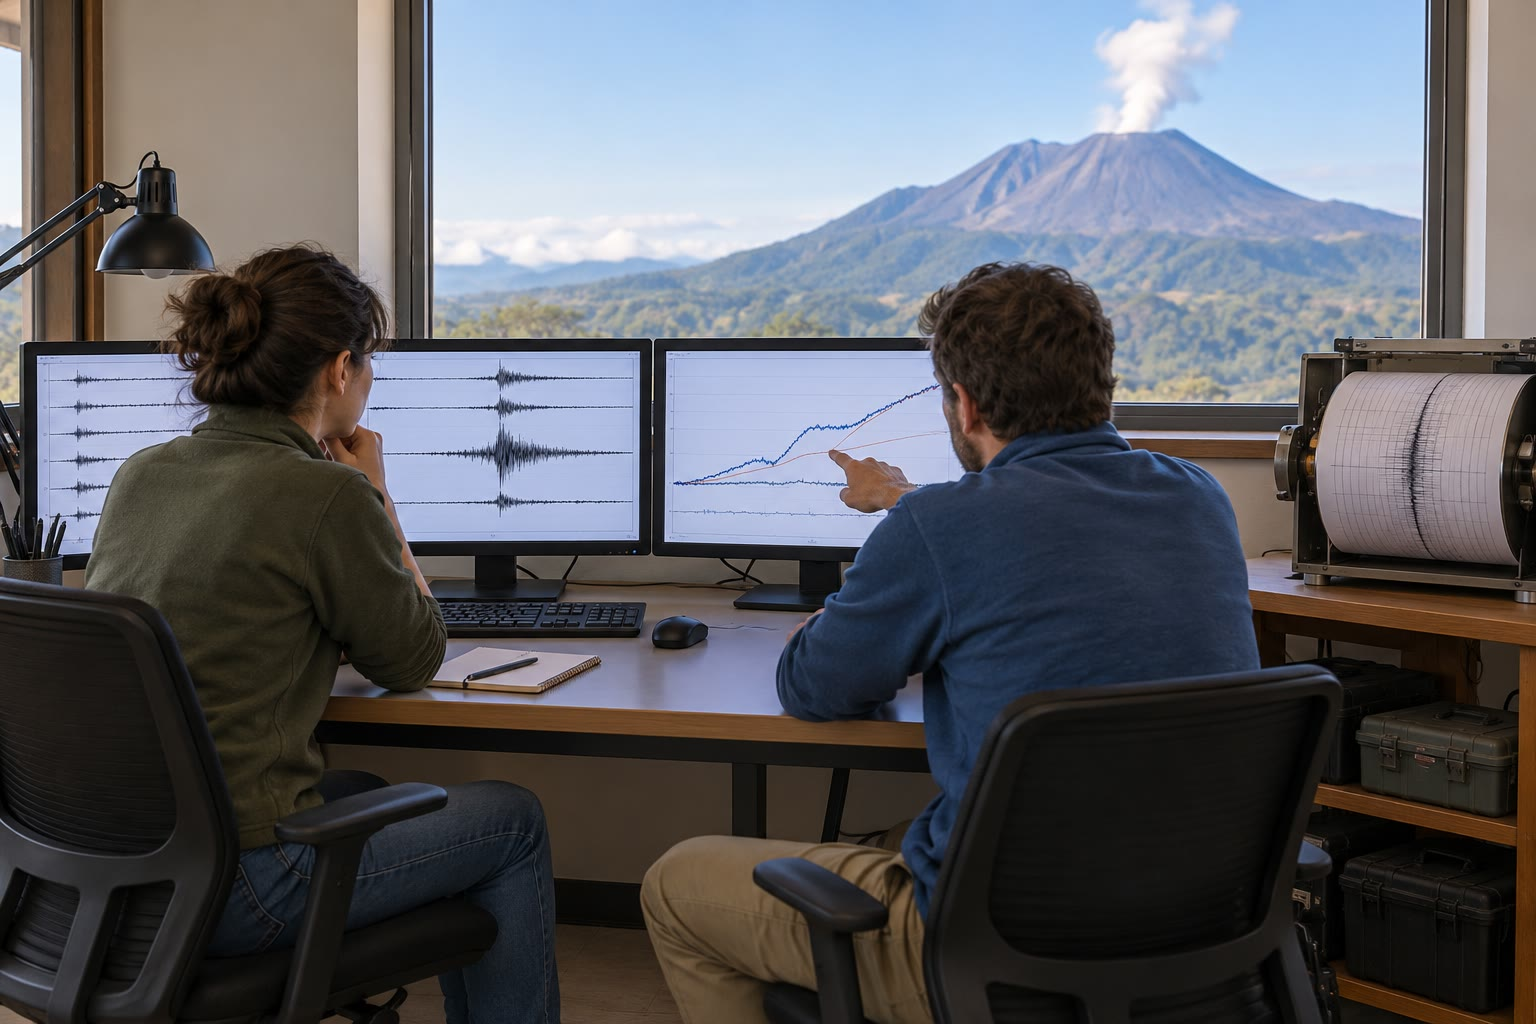
\includegraphics[width=\linewidth]{images/book4/ai/b2-volcano-observatory.jpg}
\par\smallskip{\scriptsize एक ज्वालामुखी वेधशाला में भूकंपीय अभिलेखों की समीक्षा करते
वैज्ञानिक (AI से बनाया गया चित्रण)।}
\end{minipage}
\end{inthefield}
% ledger: hvo:alert-levels

\section{अभ्यास}

\begin{exercise}[$\star$]\label{exo:b2:eruptive-styles:1}
केवल \omterm{def:b2:eruptive-styles:tephra}{टेफ़्रा} के स्थूल आयतन से सूचित VEI बताइए: (क) माउंट सेंट~हेलेंस की
राख, 18 मई 1980, \qty{1.3}{km^3}; (ख) कोटोपैक्सी का परत~5 अवपात,
\qty{0.29}{km^3}; (ग) \qty{2e6}{m^3} का एक छोटा उद्गार। (घ) 1991 में पिनातूबो
द्वारा फेंका गया पदार्थ ``\qty{5}{km^3} से अधिक'' बताया जाता है, फिर भी
उद्गार VEI~6 आँका गया है। वह आँकलन कम-से-कम कितना स्थूल आयतन सूचित करता है?
\end{exercise}
% ledger: usgs:vei-criteria, usgs:msh-1980-ash, biass19:layer5, usgs:pinatubo-1991

\begin{exercise}[$\star$]\label{exo:b2:eruptive-styles:2}
हर \omterm{def:b2:eruptive-styles:tephra}{पायरोक्लास्ट} का नाम बताइए: (क) \qty{0.5}{mm} लंबा काँच का एक कतरा; (ख) \qty{3}{cm}
चौड़ा झाँवे का एक खंड; (ग) \qty{20}{cm} चौड़ा पुराने लावा का एक कोणीय
टुकड़ा; (घ) ऐंठे सिरों वाला \qty{8}{cm} लंबा तकुए जैसा लोंदा।
\end{exercise}
% ledger: nps:pyroclast-sizes

\begin{exercise}[$\star$]\label{exo:b2:eruptive-styles:3}
$H = 0.304\,Q^{0.241}$ के साथ ($H$ छिद्र के ऊपर किलोमीटर में, $Q$
\unit{kg/s} में): (क) $H$ परिकलित कीजिए, $Q = \qty{e6}{kg/s}$ और \qty{e8}{kg/s} के लिए;
(ख) \qty{35}{km} ऊँचे स्तंभ से सूचित द्रव्यमान उद्गार-दर परिकलित कीजिए, और उसकी
तीव्रता $I = \log_{10}Q + 3$; (ग) यदि मापी गई
ऊँचाई \qty{20}{\percent} अधिक हो तो $Q$ किस गुणक से बदलता है?
\end{exercise}
% ledger: aubry23:fits, brown14:record

\begin{exercise}[$\star$]\label{exo:b2:eruptive-styles:4}
कोटोपैक्सी के परत~5 अवपात का स्थूल आयतन \qty{0.29}{km^3} है। निक्षेप का
स्थूल घनत्व \qty{1000}{kg/m^3} और \omterm{def:b2:magma-emplacement:magma}{मैग्मा} का \qty{2500}{kg/m^3} मानकर,
उसका सघन-शैल समतुल्य आयतन, उसका द्रव्यमान और उसका परिमाण
$M = \log_{10}m - 7$ परिकलित कीजिए।
\end{exercise}
% ledger: biass19:layer5, brown14:record

\begin{exercise}[$\star\star$]\label{exo:b2:eruptive-styles:5}
एक अवपात-निक्षेप $\sqrt A = \qty{5}{km}$ की समस्थूलता-रेखा पर \qty{40}{cm} मोटा है
और $\sqrt A = \qty{15}{km}$ वाली पर \qty{10}{cm}, और एक अकेले
चरघातांक के रूप में पतला होता है। $k$, $T_0$, मोटाई-अर्धदूरी $\ln 2/k$, स्थूल
आयतन और VEI परिकलित कीजिए।
\end{exercise}

\begin{exercise}[$\star\star$]\label{exo:b2:eruptive-styles:6}
(क) दिखाइए कि समस्थूलता-रेखा $x = \sqrt A$ के भीतर का आयतन, $T_0e^{-kx}$ के रूप में पतले होते
निक्षेप के लिए, $\frac{2T_0}{k^2}[1 - (1 + kx)e^{-kx}]$ है। (ख) $(1 + u)e^{-u} =
1/2$ को बार-बार प्रतिस्थापन या द्विभाजन से तीन सार्थक अंकों तक हल कीजिए। (ग)
\cref{exo:b2:eruptive-styles:5} के निक्षेप के लिए, आधा आयतन किस समस्थूलता-रेखा से परे पड़ता है? इसकी तुलना
मानचित्रित की गई सबसे बाहरी समस्थूलता-रेखा की छिद्र से दूरी से कीजिए।
\end{exercise}

\begin{exercise}[$\star\star$]\label{exo:b2:eruptive-styles:7}
\qty{850}{\celsius} (\qty{1123}{K}) पर एक रायोलाइटी \omterm{def:b2:magma-emplacement:magma}{मैग्मा} में
\qty{5.0}{\percent} जल है, विलेयता $s = 0.444$ प्रतिशत प्रति
$\sqrt{\unit{MPa}}$ के साथ; उसके गलित का घनत्व \qty{2300}{kg/m^3} है। (क) उसका
संतृप्ति दाब परिकलित कीजिए, और वह गहराई जहाँ यह \qty{0.025}{MPa/m} की
दाब-प्रवणता के लिए प्राप्त होता है। (ख) यदि गैस \omterm{def:b2:magma-emplacement:magma}{मैग्मा} में रहे तो
\qty{10}{MPa} पर गैस का आयतन-अंश परिकलित कीजिए ($R = \qty{8.314}{J/(mol.K)}$, $M =
\qty{0.018015}{kg/mol}$)। (ग) बेसाल्टी \omterm{def:b2:magma-emplacement:magma}{मैग्मा} इतने कम बार क्यों विखंडित होते हैं,
जबकि \qty{1}{MPa} पर \qty{1}{\percent} जल वाला बंद-तंत्र बेसाल्ट
\qty{92}{\percent} गैस होता?
\end{exercise}
% ledger: moore98:h2o, cassidy18:fragmentation, cassidy18:ascent

\begin{exercise}[$\star\star$]\label{exo:b2:eruptive-styles:8}
(क) \qty{5}{km} गहराई पर एक \omterm{prop:b2:eruptive-styles:mogi}{मोगी स्रोत} \qty{e7}{m^3} बढ़ता है। उसके ऊपर का
उत्थान परिकलित कीजिए ($\nu = 0.25$)। (ख) एक अन्य उभार अपने केंद्र से \qty{3.8}{km} पर
अपने अधिकतम के आधे तक गिर जाता है: उसका स्रोत कितना गहरा है? (ग) स्रोत की गहराई के बराबर
क्षैतिज दूरी पर स्थित केंद्र अधिकतम उत्थान का कितना अंश देखता
है?
\end{exercise}
% ledger: dmodels:mogi

\begin{exercise}[$\star\star$]\label{exo:b2:eruptive-styles:9}
एक वल्कनियन विस्फोट क्रेटर से खंड बाहर फेंकता है। वायु-प्रतिरोध
और क्रेटर-किनारे की ऊँचाई की उपेक्षा करके,
\qty{100}{m/s}, फिर \qty{200}{m/s} पर प्रक्षेपित खंड का अधिकतम परास परिकलित कीजिए ($g = \qty{9.81}{m/s^2}$)। क्या वायु-प्रतिरोध
इन परासों को ऊपरी सीमा बनाता है या निचली? छिद्र के चारों ओर
प्राक्षेपिक संकट का क्षेत्र प्रक्षेपण-चाल के वर्ग के अनुसार क्यों बढ़ता है?
\end{exercise}

\begin{exercise}[$\star\star\star$]\label{exo:b2:eruptive-styles:10}
(क) विधि-बॉक्स में दिए गए दो चरघातांकी खंडों वाले निक्षेप का आयतन व्युत्पन्न कीजिए,
यह मानकर कि जहाँ रेखाएँ काटती हैं वहाँ मोटाई सतत है। (ख)
कोटोपैक्सी के परत~5 अवपात के लिए, बिठाए गए खंड $T = \qty{1285}{cm}\times
e^{-0.365x}$ और ढाल $k_2 = \qty{0.138}{km^{-1}}$ वाला एक दूरस्थ खंड हैं, जो
$X = \qty{8.56}{km}$ पर काटते हैं। आयतन, और उसका वह हिस्सा जो प्रतिच्छेद-बिंदु से
परे है, परिकलित कीजिए।
\end{exercise}
% ledger: biass19:layer5

\begin{exercise}[$\star\star\star$]\label{exo:b2:eruptive-styles:11}
(क) \cref{prop:b2:eruptive-styles:plume} का प्रयोग
करके बताइए कि उद्गार-दर को 100 से गुणा करने पर
स्तंभ की ऊँचाई किस गुणक से बढ़ती है। आनुभविक घातांकों $0.241$ और $0.226$ से तुलना कीजिए।
(ख) अधिक प्रबलता से स्तरित वायुमंडल ऊँचाई को किस दिशा में बदलता है, और यदि $N$
\qty{20}{\percent} बढ़े तो कितना? (ग) दो कारण बताइए कि मापे गए घातांक
$1/4$ से नीचे क्यों पड़ सकते हैं।
\end{exercise}
% ledger: aubry23:fits

\begin{exercise}[$\star\star\star$]\label{exo:b2:eruptive-styles:12}
वैश्विक सूची VEI~4 या अधिक के 132 उद्गार सूचीबद्ध करती है जो 1500
और 1899 के बीच शुरू हुए, और 1900 और 2024 के बीच 95। (क) हर अवधि में प्रति शताब्दी दर
परिकलित कीजिए। (ख) यदि 1900 से की दर वास्तविक है, तो पहले के
उद्गारों का कितना अंश दर्ज हुआ? (ग) बड़े उद्गारों का एक अध्ययन 1500 और 1900 के बीच
परिमाण 4 से 4.9 के 21 उद्गार प्रति शताब्दी पाता है और 1900 से 56; तुलना कीजिए।
(घ) यह अंश उद्गारों के आकार पर क्यों निर्भर करता है?
\end{exercise}
% ledger: data:b4-gvp-eruptions, brown14:record

\section{समस्या: एक प्लिनियन निक्षेप को पढ़ना}

\begin{problem}[{सप्ताहांत समस्या --- झाँवे के एक अवपात की समस्थूलता-रेखाओं से उसके उद्गार के
आकार, उसके स्तंभ की ऊँचाई, और ऐसे उद्गार कितनी बार
होते हैं, तक}]
\label{pb:b2:eruptive-styles:1}
एक काल्पनिक ज्वालामुखी ने एक अकेले प्लिनियन चरण से झाँवे का एक अवपात छोड़ा है जो
\qty{10}{\hour} चला। उसकी समस्थूलता-रेखाएँ, उनके क्षेत्रफलों के वर्गमूल का प्रयोग करके
हवा से हुई दीर्घता हटाने के बाद, ये हैं:
\begin{center}
\small
\begin{tabular}{lccccc}
\hline
$\sqrt A$ (\unit{km}) & 10 & 20 & 40 & 80 & 120 \\
मोटाई $T$ (\unit{cm}) & 200 & 100 & 48 & 14 & 4.0 \\
\hline
\end{tabular}
\end{center}
डेटा: निक्षेप का स्थूल घनत्व \qty{900}{kg/m^3}; \omterm{def:b2:magma-emplacement:magma}{मैग्मा} का घनत्व
\qty{2400}{kg/m^3}; सबसे बड़े खंडों से मापी गई स्तंभ की ऊँचाई,
छिद्र के ऊपर \qty{31}{km}; क्षोभसीमा \qty{16}{km} पर। $H =
0.304\,Q^{0.241}$ और $H = 0.345\,Q^{0.226}$ का प्रयोग कीजिए ($H$ किलोमीटर में, $Q$
\unit{kg/s} में)।

\medskip\noindent\textbf{भाग I --- निक्षेप।}
\begin{enumerate}
\item हर समस्थूलता-रेखा के लिए $\ln T$ परिकलित कीजिए और दिखाइए कि $\sqrt A$ के सापेक्ष आलेखित करने पर
बिंदु दो सीधे खंडों पर पड़ते हैं। विराम कहाँ है?
\item पहली दो समस्थूलता-रेखाओं से होकर जाते निकटस्थ खंड की ढाल $k_1$ और
अंतःखंड $T_0$ परिकलित कीजिए।
\item तीन दूरस्थ समस्थूलता-रेखाओं से होकर न्यूनतम-वर्ग रेखा $T =
\qty{167}{cm}\times e^{-0.0311\sqrt A}$ है। जाँचिए कि यह उनमें से हर एक के
\qty{5}{\percent} के भीतर से गुज़रती है।
\item $\sqrt A$ का वह मान परिकलित कीजिए जिस पर दोनों रेखाएँ काटती हैं।
\item दोनों खंडों की मोटाई-अर्धदूरियाँ $\ln 2/k$ परिकलित कीजिए।
\item वह आयतन परिकलित कीजिए जो निक्षेप का होता यदि वह हर जगह निकटस्थ
ढाल के साथ पतला होता।
\item दोनों खंडों के साथ स्थूल आयतन परिकलित कीजिए, और वह हिस्सा जो
धीमे दूरस्थ खंड के संशोधन से आता है।
\item यदि केवल निकटस्थ निक्षेप मानचित्रित किया गया होता, तो आयतन किस गुणक से कम आँका
जाता? पुराने निक्षेपों के लिए यह वास्तविक जोखिम क्यों है?
\end{enumerate}

\noindent\textbf{भाग II --- उद्गार का आकार।}
\begin{enumerate}[resume]
\item उद्गार का VEI बताइए।
\item सघन-शैल समतुल्य आयतन परिकलित कीजिए।
\item उद्गारित द्रव्यमान परिकलित कीजिए।
\item परिमाण $M = \log_{10}m - 7$ परिकलित कीजिए।
\item यह निक्षेप 1980 में माउंट सेंट~हेलेंस के राख-अवपात,
\qty{1.3}{km^3}, से कितने गुना बड़ा है?
\item VEI सारणी इस उद्गार के साथ कौन-सी स्तंभ-ऊँचाई जोड़ती है, और
कौन-सी शैली?
\end{enumerate}

\noindent\textbf{भाग III --- स्तंभ।}
\begin{enumerate}[resume]
\item प्लिनियन चरण पर माध्य द्रव्यमान उद्गार-दर परिकलित कीजिए, और उसकी
तीव्रता $I = \log_{10}Q + 3$।
\item पहले आनुभविक नियम द्वारा पूर्वानुमानित स्तंभ-ऊँचाई परिकलित कीजिए।
\item दूसरे नियम से यही।
\item नियमों के प्रकीर्णन को देखते हुए, खंडों से मापे गए \qty{31}{km} से
तुलना कीजिए।
\item पहले नियम से \qty{31}{km} कौन-सी द्रव्यमान उद्गार-दर सूचित करेगा? यह प्रश्न~15 की दर से
किस गुणक से भिन्न है, और इसे क्या समझा सकता है?
\item क्या स्तंभ ने समतापमंडल में गैस पहुँचाई? जलवायु के लिए इसका क्या परिणाम
हो सकता है, और मुख्य गैस कौन-सी होगी?
\end{enumerate}

\noindent\textbf{भाग IV --- कितनी बार?}
\begin{enumerate}[resume]
\item सूची की गणनाओं से (1950 से
2024 तक VEI $\ge 3$ के 399 उद्गार, 1900 से VEI $\ge 4$ के 95, 1800 से VEI $\ge 5$ के 22,
1500 से VEI $\ge 6$ के 8, सभी खिड़कियाँ 2024 सहित समाप्त), चारों वार्षिक दरें और
उनके लघुगणक परिकलित कीजिए।
\item जाँचिए कि रेखा $\log_{10}\lambda_v = 3.28 - 0.85\,v$ हर दर के
\qty{10}{\percent} के भीतर से गुज़रती है।
\item बड़े उद्गारों के लिए हर खिड़की और पीछे से क्यों शुरू होती है?
\item रेखा से VEI $\ge 5$ के उद्गारों की दर, उनका माध्य
पुनरावृत्ति काल, और अगले 10 वर्षों में कम-से-कम एक की प्रायिकता परिकलित कीजिए।
\item रेखा से VEI $\ge 7$ के उद्गारों की दर परिकलित कीजिए और उसकी तुलना
वर्ष 1000 से दर्ज दो से कीजिए।
\item रेखा से VEI $\ge 6$ के उद्गारों की दर, और अगले 100
वर्षों में पृथ्वी पर कहीं कम-से-कम एक की प्रायिकता, प्रतिशत में, परिकलित कीजिए, जो इस
समस्या की मुख्य संख्या है। यह किस धारणा पर टिकी है?
\end{enumerate}
\end{problem}
